\documentclass[preview]{standalone}

\usepackage{amsmath}
\usepackage{amssymb}
\usepackage{stellar}
\usepackage{definitions}
\usepackage{tikz}

\usetikzlibrary{arrows.meta, decorations.markings, positioning}

\begin{document}

\id{homology-introduction}
\genpage

\section{Simplices and Simplicial Complexes}

\begin{snippetdefinition}{n-simplex-definition}{\(n\)-simplex}
    The \emph{\(n\)-simplex} \(\Delta^n\)
    is the convex hull of \(n+1\) affinely independent points
    in some Euclidean space.
\end{snippetdefinition}

\begin{snippet}{n-simplex-illustration}
    \begin{center}
        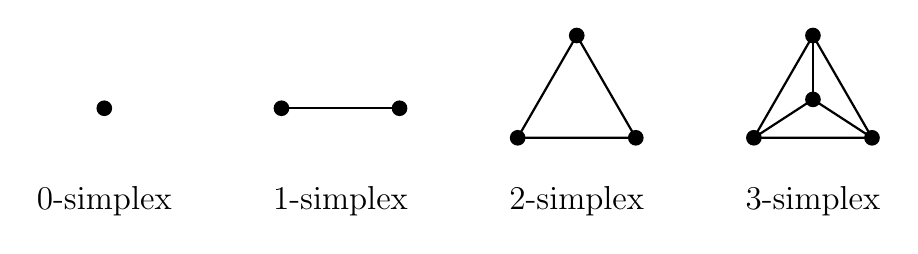
\begin{tikzpicture}[
            scale=0.75,
            % Stile per i vertici (pallini neri)
            vertex/.style={circle, fill=black, inner sep=2pt},
            % Stile per le linee (bordi)
            edge/.style={thick, black},
            % Stile per le etichette di testo
            label/.style={below=0.5cm, font=\large}
        ]

            % --- 0-simplesso (Punto) ---
            \node[vertex] (p0) at (0, 0.5) {};
            \node[label] at (0, 0) {0-simplex};

            % --- 1-simplesso (Linea) ---
            \begin{scope}[xshift=3cm]
                \coordinate (a) at (0, 0.5);
                \coordinate (b) at (2, 0.5);
                
                \draw[edge] (a) -- (b);
                \node[vertex] at (a) {};
                \node[vertex] at (b) {};
                \node[label] at (1, 0) {1-simplex};
            \end{scope}

            % --- 2-simplesso (Triangolo) ---
            \begin{scope}[xshift=7cm]
                \coordinate (a) at (0, 0);
                \coordinate (b) at (2, 0);
                \coordinate (c) at (1, 1.732); % Altezza triangolo equilatero
                
                \draw[edge] (a) -- (b) -- (c) -- cycle;
                
                \node[vertex] at (a) {};
                \node[vertex] at (b) {};
                \node[vertex] at (c) {};
                \node[label] at (1, 0) {2-simplex};
            \end{scope}

            % --- 3-simplesso (Tetraedro) ---
            \begin{scope}[xshift=11cm]
                % Vertici esterni
                \coordinate (a) at (0, 0);
                \coordinate (b) at (2, 0);
                \coordinate (c) at (1, 1.732);
                % Vertice centrale (proiezione 3D)
                \coordinate (d) at (1, 0.65); 
                
                % Disegna i bordi esterni
                \draw[edge] (a) -- (b) -- (c) -- cycle;
                % Disegna i bordi interni verso il centro
                \draw[edge] (a) -- (d);
                \draw[edge] (b) -- (d);
                \draw[edge] (c) -- (d);
                
                % Disegna i pallini
                \foreach \point in {a,b,c,d}
                    \node[vertex] at (\point) {};
                    
                \node[label] at (1, 0) {3-simplex};
            \end{scope}

        \end{tikzpicture}
    \end{center}
\end{snippet}

\begin{snippetdefinition}{k-face-simplex-definition}{\(k\)-face}
    A \emph{\(k\)-face} of an \(n\)-simplex is a subset of the \set of vertices of
    \(\simplex^n\) with order \(k+1\).
    The faces of an \(n\)-simplex with dimension less than \(n\) are called
    its \emph{proper faces}.
\end{snippetdefinition}

\begin{snippetdefinition}{properly-situated-simplices-definition}{Properly situated simplices}
    Two simplices are said to be \emph{properly situated}
    if their intersection is either empty or a face of
    both simplices.
\end{snippetdefinition}

\plain{By identifying simplices along their faces, we get a simplicial complex.}

\begin{snippetdefinition}{simplicial-complex-definition}{Simplicial complex}
    A \emph{simplicial complex} \(K\) is a finite \set of simplices such that:
    \begin{enumerate}
        \item if \(\alpha\) is a face of \(A\in K\), then \(\alpha \in K\);
        \item if \(A,B\in K\), then \(A\) and \(B\) are properly situated.
    \end{enumerate}
\end{snippetdefinition}

\begin{snippetdefinition}{simplicial-complex-dimension-definition}{Simplicial complex dimension}
    The \emph{dimension} of a simplicial complex is the maximum
    dimension of the simplices in it.
\end{snippetdefinition}

\begin{snippet}{simplicial-complex-realization}
    Given a simplicial complex \(K\), we may assign to it a \emph{geometric realization}.
    If \(K\) has vertices \(v_0, v_1, \dots, v_k\), there are many ways to assign a point
    in Euclidean space to each vertex and hence realize \(K\) geometrically.
    A convenient choice is to embed \(K\) in \(\realnumbers^k\) by assigning each vertex
    \(v_i\) to the \(i\)-th standard basis vector \(e_i\).
    Any two geometric realizations of \(K\) are homeomorphic.
    However, in general, if \(K\) is \(n\)-dimensional, it need not admit a realization
    in \(\realnumbers^n\); higher-dimensional Euclidean space may be required.
\end{snippet}

\begin{snippetdefinition}{simplex-orientation-definition}{Simplex orientation}
    An \emph{orientation} on a simplex \(\sigma = [v_0, v_1, \cdots, v_n]\)
    is an \equivrelation of ordering of its vertices,
    where two orderings \((v_0, \cdots, v_n)\) and \((w_0, \cdots, w_n)\)
    are equivalent if the permutation \(\pi\) such that
    \[
        w_i = v_{\pi(i)}
    \]
    is even.
\end{snippetdefinition}

\begin{snippetexample}{simplex-orientation-example}{}
    Reversing the orientation of a simplex is written as
    \[
        -[v_0, v_1, \cdots, v_n] = [v_1, v_0, v_2, \cdots, v_n]
    \]
    The orientation is also equivalent to the sign of
    \[
        \det(e_1 - e_0, \cdots, e_n - e_0)
    \]
    where \((e_0, \cdots, e_n)\) is a geometric realization of the simplex.
\end{snippetexample}

\begin{snippetexample}{simplex-orientation-example2}{}
    Given a \(2\)-simplex and the orientation \((v_0, v_1, v_2)\),
    we also have an induced orientation on its \(1\)-faces.
    That is, \(e_2 = (v_0, v_1), e_0 = (v_1, v_2), e_1 = (v_2, v_0)\).
    \begin{center}
        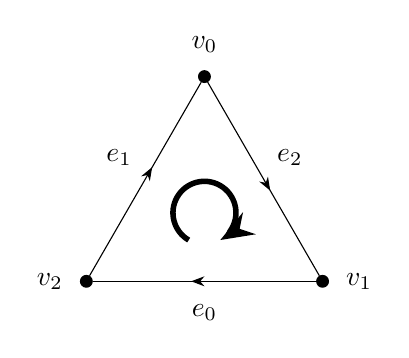
\begin{tikzpicture}[
            >=Stealth,
            node distance=3cm,
            vertex/.style={circle, draw, fill=black, inner sep=1.5pt},
            oriented/.style={decoration={markings,mark=at position 0.5 with {\arrow{>}}},postaction={decorate}},
            oriented_reversed/.style={decoration={markings,mark=at position 0.5 with {\arrow{<}}},postaction={decorate}}
        ]

        % Definizione dei vertici
        \node[vertex] (v0) at (1.5, 2.6) {};
        \node[vertex] (v1) at (3, 0) {};
        \node[vertex] (v2) at (0, 0) {};

        % Etichette dei vertici
        \node[above=5pt] at (v0) {$v_0$};
        \node[right=5pt] at (v1) {$v_1$};
        \node[left=5pt] at (v2) {$v_2$};

        % Lati con orientazione
        \draw[oriented_reversed] (v2) -- node[below=5pt] {$e_0$} (v1);
        \draw[oriented_reversed] (v1) -- node[above right=2pt] {$e_2$} (v0);
        \draw[oriented_reversed] (v0) -- node[above left=2pt] {$e_1$} (v2);

        % Freccia di orientazione centrale
        \node (center) at (1.5, 0.87) {};
        \draw[->, line width=2pt] (center) ++(240:0.4cm) arc (240:-60:0.4cm);

        \end{tikzpicture}
    \end{center}
\end{snippetexample}

\begin{snippet}{simplex-orientation-faces}
    If \(\sigma = [v_0, \cdots, v_n]\) is oriented,
    then its \(i\)-th face inherits the orientation
    \[
        (-1)^{i}[v_0, \cdots, v_{i-1}, v_{i+1}, \cdots, v_n]
    \]
\end{snippet}

\section{Homology}

\plain{We want to use simplices to convert information about shape (holes and such)
into algebraic structures.}

\begin{snippetdefinition}{n-chain-definition}{\(n\)-chain}
    Let \(K\) be a finite simplicial complex and \(G\) an abelian \group.
    An \emph{\(n\)-chain} is defined as
    \[ \sum_{i=1}^k g_i \sigma_i \]
    where \(g_i \in G\) and \(\sigma_i \in K\) oriented \(n\)-simplices.
\end{snippetdefinition}

\begin{snippetdefinition}{n-chain-group-definition}{Group of \(n\)-chains}
    Let \(K\) be a finite simplicial complex and \(G\) an abelian \group.
    The \set of \(n\)-chains forms a \group \(C_n(K; G)\) with the operation
    \[
        \left(\sum_{i=1}^k g_i \sigma_i\right)
        +
        \left(\sum_{i=1}^k h_i \sigma_i\right)
        \triangleq
        \sum_{i=1}^k (g_i + h_i) \sigma_i
    \]
\end{snippetdefinition}

\plain{This group is always abelian. Usually the additive integer group is used.}

\begin{snippetdefinition}{n-chain-boundary-operator-definition}{Boundary operator}
    Let \(K\) be a finite simplicial complex and \(G\) an abelian \group. \\
    The \emph{boundary operator} \(\partial_n \colon C_n(K;G) \fromto C_{n-1}(K;G)\)
    is defined on oriented \(n\)-simplices as
    \[
        \partial_n[v_0, v_1, \cdots, v_n] \triangleq
        \sum_{i=0}^n {(-1)}^i [v_0, \cdots, v_{i-1}, v_{i+1}, \cdots, v_n]
    \]
    and extended on \(n\)-chains as
    \[
        \partial_n \left(
            \sum_{i=1}^k g_i \sigma_i
        \right) \triangleq
        \sum_{i=1}^k g_i \partial_n(\sigma_i)
    \]
    where \(g_i \in G\) and \(\sigma_i \in K\) oriented \(n\)-simplices.
\end{snippetdefinition}

\begin{snippetexample}{boundary-operator-example}{}
    Consider the oriented \(2\)-simplex \([v_0, v_1, v_2]\).
    Its oriented \(1\)-faces are
    \[
        e_0 = [v_1, v_2], \quad
        e_1 = [v_2, v_0], \quad
        e_2 = [v_0, v_1].
    \]
    We have
    \begin{align*}
        \partial_1(\partial_2 [v_0, v_1, v_2])
        &= \partial_1(e_0 + e_1 + e_2) \\
        &= \partial_1 e_0 + \partial_1 e_1 + \partial_1 e_2 \\
        &= ([v_2] - [v_1]) + ([v_0] - [v_2]) + ([v_1] - [v_0]) \\
        &= 0
    \end{align*}
\end{snippetexample}

\plain{The boundary of a boundary is always zero.}

\begin{snippettheorem}{boundary-operator-fundamental-property}{Fundamental property of boundary operator}
    Let \(K\) be a finite simplicial complex and \(G\) an abelian \group.
    \[
        \partial_{n-1} \circ \partial_n = 0
    \]
\end{snippettheorem}

\begin{snippetdefinition}{simplicial-cycle-definition}{Cycle}
    Let \(K\) be a finite simplicial complex and \(G\) an abelian \group.
    An \emph{\(n\)-cycle} is an \(n\)-chain with
    zero boundary
    \[
        Z_n(K; G) \triangleq \grpker \partial_n = \{c \in C_n(K; G) \suchthat \partial_n c = 0 \}
    \] 
\end{snippetdefinition}

\begin{snippetdefinition}{simplicial-boundary-definition}{Boundary}
    Let \(K\) be a finite simplicial complex and \(G\) an abelian \group.
    A \emph{boundary} is an \(n\)-chain that is the boundary
    of something higher-dimensional
    \[
        B_n(K; G) \triangleq \image \partial_{n+1} = \{
            c \in C_n(K; G) \suchthat \exists d \in C_{n+1}(K; G), \partial_{n+1} d = c
        \}
    \]
\end{snippetdefinition}

\plain{By the fundamental property of the boundary operator, every boundary is a cycle.}

\begin{snippetdefinition}{homology-group-definition}{Homology group}
    Let \(K\) be a finite simplicial complex and \(G\) an abelian \group.
    The \emph{\(n\)-homology group} is defined as
    \[
        H_n(K; G) \triangleq \frac{Z_n(K; G)}{B_n(K; G)}
        = \frac{
            \grpker \partial_n
        }{
            \image \partial_{n+1}
        }
    \]
\end{snippetdefinition}

\begin{snippet}{homology-group-expl}
    Every cycle is a potential ``hole''.
    If the cycle is also a boundary, meaning that is surrounds
    a filled surface of the complex, then the hole is ``plugged'',
    which is trivial. Otherwise, the cycle surrounds a truly empty hole.
    This is why we take the quotient.
\end{snippet}

\section{Singular homology}



% ref
% https://www.math.uchicago.edu/~may/VIGRE/VIGRE2007/REUPapers/FINALFULL/Nadathur.pdf

\end{document}